\section{Operator formalism}
In this section, we explore the quantization of the cft on a cylinder, which is related to the plane via a conformal transormation.

\subsection{Radial quantization}
On the plane, one has the freedom to choose the direction of space or time for an Euclidean theory. Here we choose the radial direction to be time and the angle direction to be space. A conformal transformation
\begin{equation}
	\xi = \frac{L}{2\pi}\log\left(z\right)
\end{equation}
maps a point $z$ on a complex palne to a point $\xi=t+ix$ on a cylinder with $t$ being the time and $x\in \rinterval[soft open fences]{0}{L}$ the space. The Hilbert space defined on the cylinder at a given time $t$ is defined within a circle with a radius $e^{2\pi t/L}$. Naturally the quantum theory defined on a cylinder can be used to understand the plane.

One can immedialy find many important properties of the radial quantization from the confromal mapping. The time evolution operator, the Hamiltonian, on a cylinder corresponds the dialation operator on the plane and the translation operator, i.e.\  the momentum, corresponds to the rotation operator on the plane. Such a quantization scheme for a cft is called radial quantization. The time ordering on a cylinder becomes radial ordering on a plane. As  a conseconce, the commutation of operators for a quantum theory is related to contour integrals through
\begin{equation}
	[A,B] = \oint_0 d\omega \oint_\omega dz \, a(z)b(\omega),
\end{equation}
where $A$ and $B$ are defined as equal time contour integral of local fields. Note that in the coutour integral, we have assumed that there is no other fields existing between the two integral circles, which means the time difference $\epsilon$ here should be infestimal small. In other words, the communicator defined here should be understood as equal-time communicator.

{\bf State-field correspondence} Following the quantum theory on a cylinder (an operator in inserted at infinit past time to the vaccum state), we define a state corresponding to the field $\phi(z,\overline{z})$
\begin{equation}
	\vert \phi \rangle = \lim_{z,\overline{z}\to 0}\phi(z,\overline{z})\vert0\rangle.
\end{equation}
Its dual state is defined as
\begin{equation}
	\langle \phi \vert = \lim_{z,\overline{z}\to 0} \overline{z}^{-2h}z^{-2\overline{h}} \langle 0 \vert \phi(1/\overline{z},1/z).
\end{equation}
It is clear that states such definied are properly normalized.

\subsection{Virasoro agebra}
With the radial quantization and state-field correspondence, one can re-express the conformal symmetry, i.e.\ the Virasoro algera conveniently.  We first introduce quantum operators for local fields and the energy-momentum tensor from equal-time contour integral (or equally mode expansion for local fields)
\begin{equation}
	\phi_n = \frac{1}{2\pi i}\oint dz \, z^{n+h-1} \phi(z),
\end{equation}
in which for the energy-momentum tensor $T(z)$ we denote its mode expansion operator as $L_n$. One then finds operators $L_n$ defind here obey Virasoro algebra using the OPE of $T(z)$ from a straightforward calculation. Again, the communicator between $L_n$ is meaningful as equal-time. One can also obtain the communicator between $L_n$ and $\phi_m$
\begin{equation}
	[L_n, \phi_m] = \left(n(h-1)-m\right) \phi_{n+m}.
\end{equation}
With the Virasoro generators $L_n$, one can also construct states as
\begin{equation}
L_{-k_1}L_{-k_2} \cdots L_{-k_n} \vert \phi \rangle.
\end{equation}

\subsection{The Free Boson}
\textit{Canonical Quantization on the Cylinder}--.
\textcolor{red}{Rewrite this part using the current operator to simplify the convention.}
Let $\phi(x,t)$ be a free Boson field defined on a cylinder of circumference $L$, such that $\phi(x+L,t) = \phi(x,t)$. The Lagrangian of the boson field is
\begin{equation}
  \mathcal{L} = \frac{1}{4\pi K}\int dx \left\{{(\partial_t\phi)}^2 - {(\partial_x \phi)}^2\right\}.
\end{equation}
Note that to connect to the convention in the previous part $g = \frac{1}{2\pi K}$.
We can Fourier transform $\phi$ as
\begin{align}
  \phi(x,t) &= \sum_n e^{\frac{2\pi}{L}inx}\phi_n(t), \\
  \phi_n(t) &= \frac{1}{L}\int dx e^{-\frac{2\pi}{L}inx}\phi(x,t).
\end{align}
The Lagrangian can be reexpressed as
\begin{equation}
  \mathcal{L} = \frac{1}{4\pi K}\sum_n\left\{\dot{\phi}_n\dot{\phi}_{-n}-{\left(\frac{2\pi n}{L}\right)}^2\phi_n\phi_{-n}\right\}.
\end{equation}
The momentum conjugate to $\phi_n$ becomes
\begin{equation}
  \pi_n = gL\dot{\phi}_{-n}, \qquad [\phi_n,\pi_m] = i\delta_{nm}.
\end{equation}
The Hamiltonian can be expressed as
\begin{equation}
  H = \frac{1}{2gL}\sum_n\{\pi_n\pi_{-n}+{(2\pi ng)}^2\phi_n\phi_{-n}\}
\end{equation}
This corresponds to a sum of decoupled harmonic oscillators with frequencies $\omega = \frac{2\pi}{L}\lvert n\rvert$.

We can introduce creation and annihalation operators, which allow the Hamiltonian to be expressed as
\begin{equation}
  H = \frac{1}{2gL}\pi_0^2+\frac{2\pi}{L}\sum_n\left(a_{-n}a_n+\overline{a}_{-n}\overline{a}_n\right).
\end{equation}

The following commutation relation holds
\begin{equation}
  [H,a_{-m}] = \frac{2\pi}{L}ma_{-m}.
\end{equation}
Applying $a_{-m}$ toan eigenstate with energy $E$, creates an eigenstate with energy $E+\frac{2\pi m}{L}$.
The Fourier modes can be expressed as
\begin{equation}
  \phi_n = \frac{i}{n\sqrt{4\pi g}}(a_n-\overline{a}_{-n})
\end{equation}
The fields can be expressed as
\begin{equation}
  \phi(x,t) = \phi_0 + \frac{1}{gL}\pi_0t + \frac{i}{\sqrt{4\pi g}}\sum_{n \neq 0}\frac{1}{n}\left(a_n e^{\frac{2\pi i}{L} n(x-t)}-\overline{a}_{-n}e^{\frac{2\pi i}{L} n(x+t)}\right).
\end{equation}
Transforming to Euclidean space, we can define the following conformal coordinates
\begin{equation}
  z = e^{\frac{2\pi}{L}(\tau-ix)}, \qquad \overline{z} = e^{\frac{2\pi}{L}(\tau+ix)}.
\end{equation}
This results in
\begin{equation}
  \phi(z,\overline{z}) = \phi_0 - \frac{i}{4\pi g}\pi_0\ln(z\overline{z}) + \frac{i}{\sqrt{4\pi g}}\sum_{n \neq 0}\frac{1}{n}\left(a_n z^{-n}+\overline{a}_{n}\overline{z}^{-n}\right).
\end{equation}
The field $\phi$ is not a primary, however the holomorphic field $\partial \phi$ is.
\begin{equation}
  i \partial \phi(z)  = \frac{\pi_0}{4\pi g z}+\frac{i}{\sqrt{4\pi g}}\sum_{n \neq 0} a_n z^{-n-1}
\end{equation}

\textit{Vertex Operators}--.
There exists an infinite variety of local fields related to $\phi$ without introducing a scale. These are called the vertex operators $\mathcal{V}_\alpha$.
\begin{equation}
  \mathcal{V}_\alpha = :e^{i\alpha\phi(z,\overline{z})}:
\end{equation}
The vertex operators have conformal dimensions $h(\alpha)=\overline{h}(\alpha) = \frac{\alpha^2}{8\pi g} = \frac{\alpha^2 K}{4}$.

\subsection{The Fock Space}
The eigenstates of $H$ can be labeled by the eigenvalues of $\pi_0$. This means that the Fock space is built upon a one-parameter family of vacua $\lvert{\alpha}\rangle$.

We know that $T(z)$ is given by
\begin{align}
  T(z) &= -2\pi g :\partial \phi(z) \partial\phi(z) :\\
  &= \frac{1}{2} \sum_{n,m}z^{-n-m-2}:a_n a_m: .
\end{align}
From this we can derive the expression for the Virasoro operators
\begin{align}
  L_n &= \frac{1}{2}\sum_{m\in\mathbb{Z}}a_{n-m}a_m \quad(n\neq 0),\\
  L_0 &= \sum_{n>0}a_{-n}a_n + \frac{1}{2}a_0^2.
\end{align}
This allows for the Hamiltonian to be expressed as
\begin{equation}
  H = \frac{2\pi}{L}(L_0+\overline{L}_0)
\end{equation}
Furthermore the elements of the Fock space $a_{-1}^{n_1}a_{-2}^{n_2}\cdots \overline{a}_{-1}^{m_1}\overline{a}_{-2}^{m_2}\cdots \lvert\alpha\rangle$ are eigenstates of $L_0$ with conformal dimensions $h=\frac{1}{2}\alpha^2+\sum_j j n_j$ and $\overline{h}=\frac{1}{2}\alpha^2+\sum_j j m_j$.
The different vacua $\lvert \alpha\rangle$ are related to the absolute vacuum $\lvert 0\rangle$ by the vertex operators $\mathcal{V}_\alpha$.\\

\noindent {\bf Twisted Boundary Conditions---}.\\
We can also assume anti-periodic boundary condition. This is compatible with the Lagrangian because it is quadratic in the fields. Changing to anti-periodic boundaries makes the summation index half-integer valued and removes the zero mode. There are now two vacua $\lvert 0_+ \rangle$ and $\lvert 0_- \rangle$.

We have that
\begin{equation}
    \langle\phi\partial\phi\rangle = \frac{1}{w}\sum_{n>0}{\left(\frac{w}{z}\right)}^n.
\end{equation}
In the periodic case the sum is over integer values and becomes
\begin{equation}
  \langle\phi\partial\phi\rangle = \frac{1}{z-w}.
\end{equation}
In the anti-periodic case the sum is over half integer values and becomes
\begin{equation}
  \langle\phi\partial\phi\rangle = \sqrt{\frac{z}{w}}\frac{1}{z-w}.
\end{equation}

For the vacuum expactation value of the energy-momentum tensor, $\langle T(z)\rangle$, we have in the periodic case $\langle T(z)\rangle = 0$, but in the anti-periodic case $\langle T(z)\rangle=\frac{1}{16z^2}$.\\

\noindent {\bf Compactified Boson}\\
We can identify $\phi$ with $\phi+2\pi R$ to get the compact boson. In general we can consider the boundary condition
\begin{equation}
  \phi(x+L,t) = \phi(x,t) + 2\pi m R,
\end{equation}
where $m$ represents the winding number of the field. This modifies the mode expansion as
\begin{equation}
  \phi(x,t) = \phi_0 + \frac{n}{gRL}t + \frac{2\pi m R}{L}x + \frac{i}{\sqrt{4\pi g}}\sum_{k\neq 0}\frac{1}{k}\left(a_k e^{\frac{2\pi i k}{L}(x-t)}-\overline{a}_{-k}e^{\frac{2\pi i k}{L}(x+t)}\right).
\end{equation}
After reexpressing in complex coordinates and taking the derivative we get
\begin{equation}
  i\partial\phi(z) = (\frac{n}{4\pi g R}+\frac{1}{2}mR)\frac{1}{z}+\frac{1}{\sqrt{4\pi g}\sum_{k\neq 0}a_k z^{-k-1}}.
\end{equation}
The virasoro operators $L_0$ and $\overline{L}_0$ can be expressed as
\begin{align}
  L_0 &= \sum_{n>0}a_{-n}a_n + 2\pi g {\left(\frac{n}{4\pi g R}+\frac{1}{2}mR\right)}^2\\
  \overline{L}_0 &= \sum_{n>0}\overline{a}_{-n}\overline{a}_n + 2\pi g {\left(\frac{n}{4\pi g R}-\frac{1}{2}mR\right)}^2
\end{align}

\subsection{The Free Fermion}
The free fermion action is given by
\begin{equation}
  S = \frac{1}{2}g\int d^2 x \Psi^\dagger\gamma^0\gamma^\mu\partial_\mu\Psi
\end{equation}
The central charge of this theory is $c=1/2$ and $\psi$ has as conformal dimension $h=1/2$.\\

\noindent {\bf Canonical Quantization on a Cylinder}\\
We can take the mode expansion of $\psi$ at $t=0$ on a cylinder with circumference $L$. This gives
\begin{equation}
  \psi(x) = \sqrt{\frac{2\pi}{L}}\sum_k b_k e^{\frac{2\pi i}{L}k x}.
\end{equation}
There are two possible types of boundary conditions. With the periodic (Ramond) boundary conditions the index k takes on integer values. With anti-periodic (Neveu-Schwarz) boundary conditions the index k must take half-integer values.

The Hamiltonian can be written as
\begin{equation}
  H = \sum_{k>0} \omega_k b_{-k}b_k +E_0, \qquad \omega_k = \frac{2\pi\lvert k\rvert}{L}.
\end{equation}\\

\noindent {\bf Mapping onto the Plane}\\
Mapping $\psi$ to the plane gives
\begin{equation}
  \psi_{cyl}(z) = \sqrt{\frac{2\pi z}{L}}\psi_{pl}(z)
\end{equation}
and thus
\begin{equation}
  \psi(z) = \sum_k b_k z^{-k-\frac{1}{2}}
\end{equation}
This transformation swaps the boundary Conditions
\begin{equation}
	\begin{aligned}
  		\psi(e^{2\pi i}z) &=-\psi(z) \qquad(Ramond)\\
  		\psi(e^{2\pi i}z) &=\psi(z) \qquad(Neveu-Schwarz)
	\end{aligned}
\end{equation}
Note that the fermion field has a dimension, which changes the boundary condition when mapped from the cylinder to the plane.

The different sectors will have a different two-point correlation function. For the NS sector we have
\begin{equation}
  \langle\psi(z)\psi(w)\rangle = \frac{1}{z-w}.
\end{equation}
In the R sector we have
\begin{equation}
  \langle\psi(z)\psi(w)\rangle = \frac{1}{2}\frac{\sqrt{z/w}+\sqrt{w/z}}{z-w}.
\end{equation}
Furthermore depending on the boundary conditions the energy-momentum tensor will gain a non-zero expectation value.
\begin{align}
  \langle T(z)\rangle &= 0 \qquad(Neveu-Schwarz)\\
  \langle T(z)\rangle &= \frac{1}{16z^2} \qquad(Ramond)
\end{align}\\


\noindent {\bf Vacuum Energies} \\
The energy momentum tensor on the plane can be written as
\begin{equation}
  T(z) = \frac{1}{2}\sum_{n,k}(k+\frac{1}{2})z^{-n-2}:b_{n-k}b_k:,
\end{equation}
which naturally leads to
\begin{equation}
  L_n = \frac{1}{2}\sum_k(k+\frac{1}{2}):b_{n-k}b_{k}:
\end{equation}
$L_0$ is given by different expressions depending on the boundary conditions.
\begin{align}
  L_0 &= \sum_{k>0}kb_{-k}b_k \qquad (NS)\\
  L_0 &= \sum_{k>0}kb_{-k}b_k + \frac{1}{16} \qquad (R)\\
\end{align}
From this we can express the Hamiltonian as
\begin{equation}
  H = \frac{2\pi}{L}(L_0 + \overline{L}_0-\frac{c}{12}).
\end{equation}





\subsection{Normal ordering}
For free fields the OPE of the field with itself contains only one term with a constant prefactor. It can be regularized by normal ordering the fields, or equivalently, subtracting its expectation value.
Using the former prescription for $T(z)T(w)$ only kills the $\propto c$ term. So clearly we need a more elaborate definition of normal ordering. We shall define proper normal ordering for general fields as subtracting all the singular terms from the OPE\@. We will write this normal ordering as
\begin{equation}
	(AB)(z).
\end{equation}
Concretely, given the OPE
\begin{equation}
	A(z)B(w) = \sum_{n=-\infty}^{N}\frac{{\left\{AB\right\}}_n(w)}{{(z-w)}^n}
\end{equation}
we have that
\begin{equation}
	(AB)(w) = {\left\{AB\right\}}_0(w).
\end{equation}
Equivalently, we can compute the normal ordering of fields using contour integral methods:
\begin{equation}
	(AB)(w) = \frac{1}{2\pi i}\oint \frac{dz}{z-w}A(z)B(w).
\end{equation}
The contraction of fields contains only the singular terms of the OPE\@:
\begin{equation}
	\wick{\c A(z) \c B(w)} = \sum_{n=1}^N\frac{{\left\{AB\right\}}_n(w)}{{(z-w)}^n}.
\end{equation}
We now want to express the modes of the normal ordered field in terms of the modes of the input fields. Given fields $A$ and $B$ and points $|z|>|x|>|w|$ we write
\begin{subequations}
\begin{align}
	A(z) &= \sum_n {(z-x)}^{-n-h_A}A_n(x) \\
	B(w) &= \sum_n {(w-x)}^{-n-h_B}B_n(x).
\end{align}
\end{subequations}
Contour integrating ultimately results in:
\begin{equation}
	{(AB)}_m = \sum_{n\leq -h_A} A_n B_{m-n} + \sum_{n>-h_A}B_{m-n}A_n,
\end{equation}
where we defined the modes of $(AB)$ as:
\begin{equation}
	{(AB)}(z) = \sum_n z^{-n-h_A-h_B}{(AB)}_n.
\end{equation}
Some warnings are in place:
\begin{enumerate}
	\item Normal ordering is not commutative: $(AB)(z) \neq (BA)(z)$.
	\item Normal ordering is not associative: $((AB)C)(z)\neq(A(BC))(z)$.
	\item With this definition of normal ordering, Wick's theorem needs to be revisited. This is done in Appendix 6.B of the Book.
\end{enumerate}

\subsection{Conformal families and Operator algebra}
\epigraph{There's nothing stronger than family.}{D. T.}

The goal of this section is to introduce the notion of conformal blocks and associated to this the method of conformal bootstrapping as a way to solve CFTs, i.e.\ compute the correlation functions, explicitly. Before that we revisit the notion of descendant fields and conformal families. In the following we mostly only care about the holomorphic part of fields.\\

\noindent{\bf Descendant fields}\\
A descendant is generated from a primary by acting with the Virasoro operators:
\begin{equation}
	\phi^{(-n)}(w) = (L_{-n}\phi)(w) = \frac{1}{2\pi i}\oint_w dz \frac{1}{{(z-w)}^{n-1}}T(z)\phi(w),
\end{equation}
in particular:
\begin{equation}
	\phi^{(0)}(w) = h\phi(w), \qquad \phi^{(-1)} = \partial \phi(w).
\end{equation}
Consider following correlation function of states that are part of the same family:
\begin{equation}
	\expval{(L_{-n}\phi)(w)X},
\end{equation}
where $X$ denotes a string of primary fields: $X=\phi_1(w_1)\cdots \phi_N(w_N)$. After a computation one finds:
\begin{equation}
	\expval{(L_{-n}\phi)(w)X} = \mathcal{L}_{-n}\expval{\phi(w)X} \qquad (n\geq 1).
\end{equation}
With the differential operator
\begin{equation}
	\mathcal{L}_{-n} = \sum_i \left\{ \frac{(n-1)h_i}{{(w_i - w)}^n} - \frac{1}{{(w_i - w)}^{n-1}}\partial_{w_i}\right\}.
\end{equation}
In other words, knowing all the correlation functions between primaries, $\expval{\phi(w)X}$, is sufficient to compute the correlation functions that involve descendants by applying the differential operators $\mathcal{L}_{-n}$. More generally, for descendants of the form
\begin{equation}
	\phi^{(-k,-n)}(w) = (L_{-k}L_{-n}\phi)(w),
\end{equation}
and so on, we find in a similar way that
\begin{equation}
	\expval{(L_{-k_1}\cdots L_{-k_n}\phi)(w)X} = \mathcal{L}_{-k_1}\cdots \mathcal{L}_{-k_n}\expval{\phi(w)X} \qquad (n\geq 1)
\end{equation}\\

\noindent {\bf Conformal families} \\
A \emph{conformal family} is a set of states that transform according to a representation of the conformal group. A family contains a primary and its descendants. We will denote the conformal family associated with the primary $\phi$ by $[\phi]$. First descendants of a primary are sometimes called \emph{secondary fields}. Another way to say that a conformal family transforms under itself is to say that the OPE of $T(z)$ with any member of the family will be composed solely of other members within the same family. Concretely:
\begin{equation}
	T(z)\phi^{(-n)}(w) = \frac{cn(n^2-1)/12}{{(z-w)}^{n+2}}\phi(w) + \sum_{k=1}^{n}\frac{n+k}{{(z-w)}^{k+2}}\phi^{(k-n)}(w) + \sum_{k\geq 0}{(z-w)}^{k-2}\phi^{(-k,-n)}(w)
\end{equation}\\

\noindent {\bf The operator algebra} \\
The two and three-point functions of a CFT are fixed by conformal invariance. However, we need additional dynamical information to compute the three-point fusion coefficients $C_{ijk}$ (for example using a conformal bootstrap approach). This information is contained in the \emph{operator algebra}. The OPE which also includes the regular terms of all primary fields with each other. Using the operator algebra we can reduce all correlation functions to two-point correlation functions.

First we choose a basis of fields such that $C_{\alpha\beta} = \delta_{\alpha\beta}$ in
\begin{equation}
	\expval{\phi_\alpha(w,\overline{w})\phi_\beta(z,\overline{z})} = \frac{C_{\alpha\beta}}{{(w-z)}^{2h}{(\overline{w}-\overline{z})}^{2\overline{h}}}.
\end{equation}
This implies that states belonging to different conformal families are always orthogonal.
From scale invariance it follows that:
\begin{equation}
	\phi_1(z,\overline{z})\phi_2(0,0) = \sum_p \sum_{\{k,\overline{k}\}} C_{12}^{p\{k,\overline{k}\}}z^{h_p-h_1 -h_2+K} \overline{z}^{\overline{h}_p-\overline{h}_1-\overline{h}_2+\overline{K}}\phi_p^{(k,\overline{k})}(0,0).
\end{equation}
We introduced the notation $K = \sum_i k_i$.

Writing
\begin{equation}
	C_{12}^{p\{0,0\}} \equiv C^p_{12} = C_{p12},
\end{equation}
we find that
\begin{equation}
	C_{12}^{p\{k,\overline{k}\}} = C_{12}^p \beta_{12}^{p\{k\}} \overline{\beta}_{12}^{p\{\overline{k}\}}.
\end{equation}
This means that descendants fields are correlated to a given third field only if the primary is correlated. An the holomorphic and antiholomorphic parts factorize.

An example is given in the Book. Even in a relatively simple case, finding the three point function is not straightforward!

In conclusion, given the central charge, the conformal dimensions and the three-point coefficients $C_{pnm}$, one can, in principle, determine the operator algebra. Using the operator algebra, all the n-point correlation functions can be computed and the entire theory is solved. \\

\noindent {\bf Conformal blocks} \\
Let us illustrate how the four-point functions can be reduced to three-point functions using the machinery introduced in the previous sections.

We consider the four-point function
\begin{equation}
	\expval{\phi_1(z_1,\overline{z}_1)\phi_2(z_2,\overline{z}_2)\phi_3(z_3,\overline{z}_3)\phi_4(z_4,\overline{z}_4)}.
\end{equation}
For sake of simplicity, we shall carry out a global conformal transformation to put $z_4 = 0$, $z_1 = \infty$, $z_2 = 1$, $z_3 = x$.
We define:
\begin{equation}
	G_{34}^{21}(x,\overline{x}) = \mel{h_1,\overline{h}_1}{\phi_2(1,1)\phi_3(x,\overline{x})}{h_4,\overline{h}_4}.
\end{equation}
Note the order of the indices!

Using operator algebra techniques, we can write this function as:
\begin{equation}
	G_{34}^{21}(x,\overline{x}) = \sum_p C_{34}^p C_{12}^p A_{34}^{21}(p|x,\overline{x}).
\end{equation}
The sum over $p$ is a sum over intermediate conformal families that play the role of mediating channels in the scattering from fields from $(0,x)$ towards $(1,\infty)$. These functions $A_{34}^{21}(p|x,\overline{x})$ are called \emph{partial waves}. They can be depicted by:
\begin{figure}[htb]
\centering
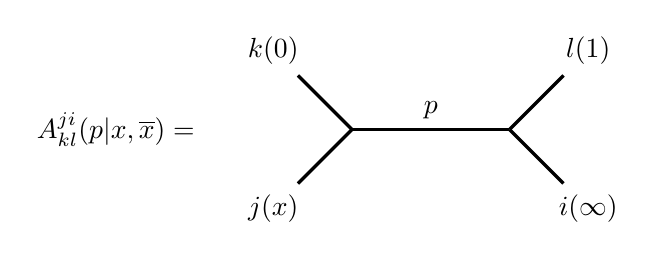
\begin{tikzpicture}[very thick]
	\node at (-1,1) (k) {$k (0)$};
	\node at (-1,-1) (j) {$j (x)$};
	\node at (3,1) (l) {$l (1)$};
	\node at (3,-1) (i) {$i (\infty)$};
	
	\node at (-3,0) {$A_{kl}^{ji}(p|x,\overline{x})=$};
	
	\draw (k) -- (0,0) ;
	\draw (j) -- (0,0);
	\draw (0,0) -- node[above] {$p$} ++ (2,0);
	\draw (2,0) -- (l);
	\draw (2,0) -- (i);
\end{tikzpicture}
\end{figure}

The partial wave factorizes in a holomorphic and antiholomorphic part, according to:
\begin{equation}
	A_{34}^{21}(p|x,\overline{x}) = \mathcal{F}_{34}^{21}(p|x)\overline{\mathcal{F}}_{34}^{21}(p|\overline{x}),
\end{equation}
we call these functions $\mathcal{F}$, the \emph{conformal blocks}. There is a recipe to compute these conformal blocks, even though it is a pain to compute these in practice. Physically speaking, these conformal blocks are the part in the four-point function that is fixed by conformal invariance. They depend on the anharmonic ratios via a series expansion. The remaining elements are the three-point coefficients, which are \emph{not} fixed by conformal invariance. \\

\noindent {\bf Crossing symmetry and the conformal bootstrap} \\
What happens if we would choose instead of $z_4 = 0$, $z_1 = \infty$, $z_2 = 1$, $z_3 = x$ a different order of the fields? Following identities can be obtained relatively easy:
\begin{equation}
	G_{34}^{21}(x,\overline{x}) = G_{32}^{41}(1-x,1-\overline{x}),
\end{equation}
and
\begin{equation}
	G_{34}^{21}(x,\overline{x}) = \frac{1}{x^{2h_3}\overline{x}^{2\overline{h}_3}}G_{31}^{24}(1/x,1/\overline{x}).
\end{equation}
These identities are specific instances of the \emph{crossing symmetry} of the functions $G$. Explicitly we can write the first identity as
\begin{equation}
	\sum_p C_{21}^p C_{34}^p\mathcal{F}_{34}^{21}(p|x)\overline{\mathcal{F}}_{34}^{21}(p|\overline{x}) = \sum_q C_{41}^q C_{32}^q \mathcal{F}_{32}^{41}(p|1-x)\overline{\mathcal{F}}_{32}^{41}(p|1-\overline{x}),
\end{equation}
which has a aesthetically pleasing pictorial interpretation:
\begin{figure}
\centering
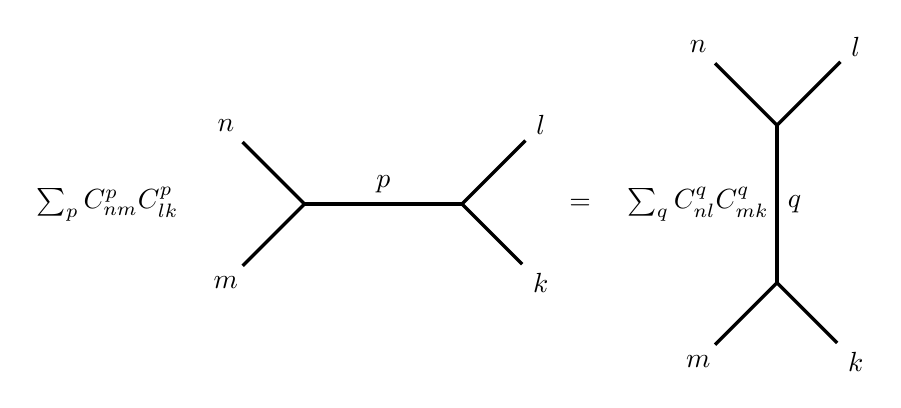
\begin{tikzpicture}[very thick]
\node at (-1,1) (k) {$n$};
\node at (-1,-1) (j) {$m$};
\node at (3,1) (l) {$l$};
\node at (3,-1) (i) {$k$};

\node at (-2.5,0) {$\sum_p C_{nm}^pC_{lk}^p$};

\draw (k) -- (0,0) ;
\draw (j) -- (0,0);
\draw (0,0) -- node[above] {$p$} ++ (2,0);
\draw (2,0) -- (l);
\draw (2,0) -- (i);

\node at (3.5,0) {$=$};

\begin{scope}[shift={(6,-1)}]
\node at (-1,-1) (m) {$m$};
\node at (1,-1) (k) {$k$};
\node at (-1,3) (n) {$n$};
\node at (1,3) (l) {$l$};

\node at (-1,1) {$\sum_q C_{nl}^qC_{mk}^q$};

\draw (m) -- (0,0) ;
\draw (k) -- (0,0);
\draw (0,0) -- node[right] {$q$} ++ (0,2);
\draw (0,2) -- (n);
\draw (0,2) -- (l);
\end{scope}
\end{tikzpicture}
\end{figure}
Crossing symmetry imposes $N^4$ constrains on the $N^3 + N$ parameters $C_{mn}^p$ and $h_p$. Exploiting crossing symmetry to compute these parameters is called \emph{conformal} bootstrap.
